Los archivos relacionados a la documentación del proyecto Voorspelling se encuentran en la carpeta \textit{Documentation} del repositorio del proyecto, la cual puede ser consultada en GitHub con el siguiente enlace: \url{https://github.com/Noczio/VoorSpelling}.

Cada carpeta contiene archivos clasificados por su tipo, ya sean diagramas, formatos, flujo de la aplicación, \textit{mockups}, \textit{sketchs} y otros recursos como el cronograma del proyecto. No obstante, los documentos que se presentan a continuación son aquellos relacionados con los requerimientos, \textit{back-end}, \textit{front-end} y casos de uso  desarrollados durante el ciclo de vida del proyecto desde Agosto del 2020 hasta Marzo del 2021.

%requerimientos
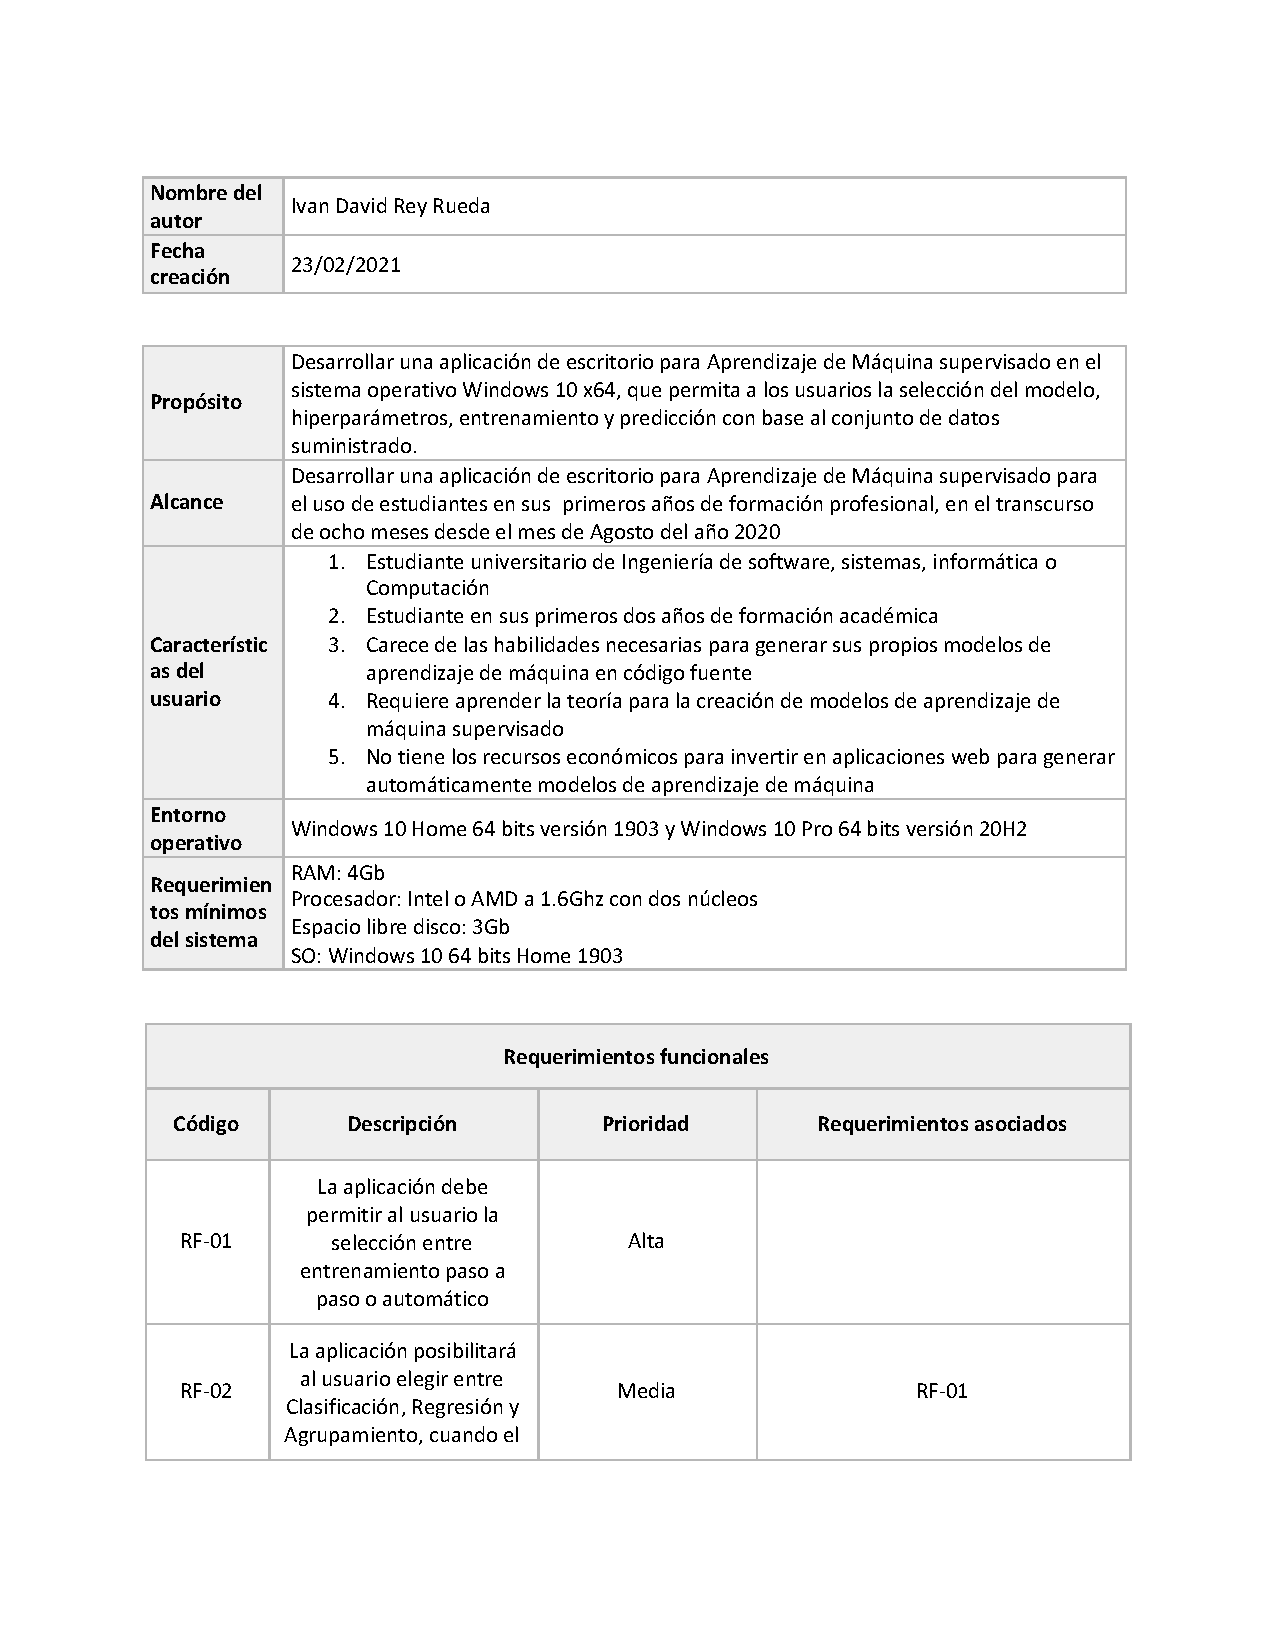
\includepdf[pages=-, pagecommand=\thispagestyle{otherplain} ,width=\textwidth]{pdfs/Requerimientos_proyecto_Firmado.pdf}